\chapter{A HIL felépítése}

\section{A hardware felépítése}

A HIL szimulátor hardware nem más, mint egy interface elektronika a vezérlő hardware-ek és a szimulációt végző FPGA között. \Afigref{hw_architect} ábrán láthatóak a vezérést végző elemek. A HIL szimulátor feladata a bal oldali, Power Subsystemb blokkból érkező jelek előállítása, illetve a vezérlő jelek fogadása. Mivel a szimuláció során a PIB nem szükséges, ezért az MCB és a CCB kapcsolatát is a HIL elektronika biztosítja

\subsection{A ZTEX kártya}

Egy iylen teszt és fejlesztési eszköz fejlesztése során az egiyk legfontosabb szempont a modularitás. Nem láthatjuk előre feltétlenül, hogy a későbbiekben mire lesz szükség. Ezen felül egy közel 500 lábbal rendelkező BGA tokos FPGA-hoz a nyáktervezés sem triviális feladat. A megfelelő lábak kivezetéséhez legalább 6-8 rétegre van szükség, és nagyon sok hibalehetőséget tartogat magában. Ezek miatt egy FPGA modul alkalmazása mellett döntöttünk. Bár az elérhető GPIO lábak mennyisége így korlátoztt, az FPGA-t működtető áramkör garantáltan működőképes, illetve a saját tervezésű elektornika bonyolultsága is jelentősen csökken.

\begin{figure}[!ht]
	\centering
	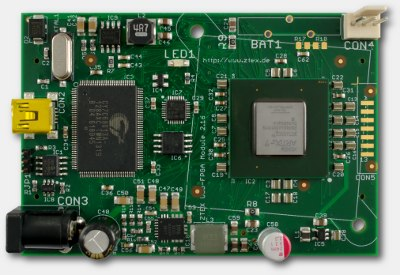
\includegraphics[width = \textwidth]{figures/fpga216.jpg}
	\caption{A ZTEX 2.16 FPGA board} 
	\label{fig:ztex}
\end{figure}

\Aref{fig:ztex} ábrán látható ZTEX panel mellett tettem le a voksom. A kártyán található egy USB-s loader, így JTAG programozó eszköz sem feltétlenül szükséges az FPGA feltöltéséshez, illetve FLASH memória is található az eszközön, így automatikusan minden indulákor betöltődik a firmware az FPGA-ba.


\begin{figure}[!ht]
	\centering
	\includegraphics[width = \textwidth]{figures/fpga216blox.jpg}
	\caption{A ZTEX 2.16 FPGA board felépítése} 
	\label{fig:ztex_block}
\end{figure}




\section{A szimulátor szerepe a folyamatban}
\section{A szimulátor felépítése}
\subsection{A hardware felépításe}
\subsection{A firmware felépítése}